\section{VQ-GAN}
\label{sec:vqgan}

\begin{figure}
    \centering
    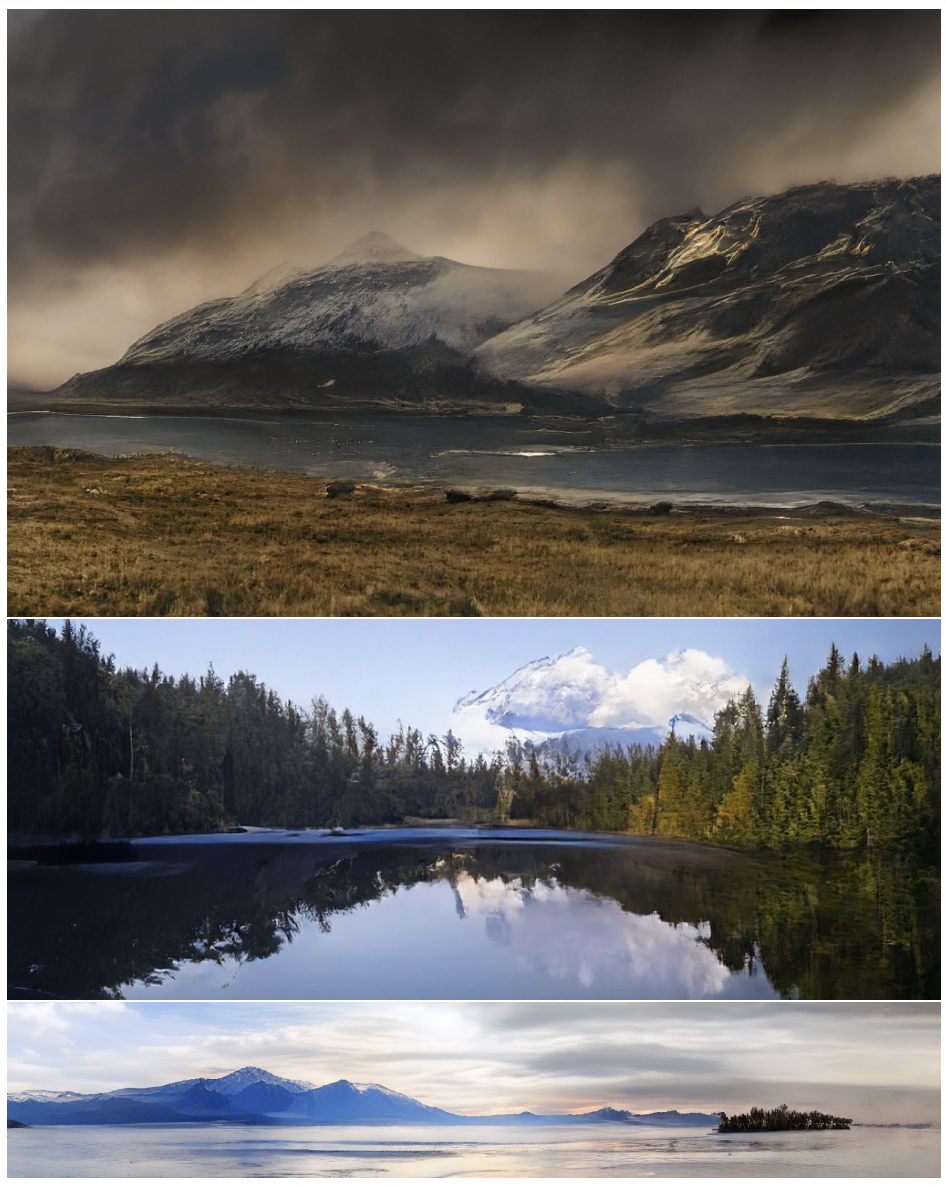
\includegraphics[width=0.5\textwidth]{images/vqgan_samples.png}
    \caption{Samples generated by VQ-GAN with different resolutions (top to bottom: 1280x832, 1024x416, 1280x240), conditioned on semantic layouts from S-FLCKR dataset.}
\end{figure}

Vector Quantized Generative Adversarial Network (VQ-GAN) \cite{vqgan} is a deep learning model capable of generating high-quality images, with the ability of conditioning (text, images, semantic masks and human pose). The architecutre of VQ-GAN is based on previous works: Vector Quantized Variational Autoencoder (VQ-VAE) \cite{vqvae} (section \ref{sec:vqvae}), transformers \cite{transformer} (appendix \ref{sec:transformers}), and Generative Adversarial Network (GAN) \cite{gan} (section \ref{sec:gan}). The main premises of VQ-GAN is instead of representing an image with pixels, they represent it as a composition of perceptually rich image constituents from a codebook.

VQ-GAN takes the best of both worlds: the ability to generate high-quality images from GANs and the ability to condition the generation process from VQ-VAE using transformers. The combination of the expressivness of transformers and the inductive bias \footnote[1]{Inductive bias is the ability to capture local information in the image, which is why CNN is chosen,  because of the pooling layers.} of CNNs \cite{cnn} in this work showed significant improvements in image generation tasks compared to previous models. Transformers can learn long-range dependencies, whereas CNNs are better fit at learning local features and structures of images. Additional benefit in using a transformer is that is allows the model to output images of various resolutions, which is not possible with previous works.

\begin{figure}
    \centering
    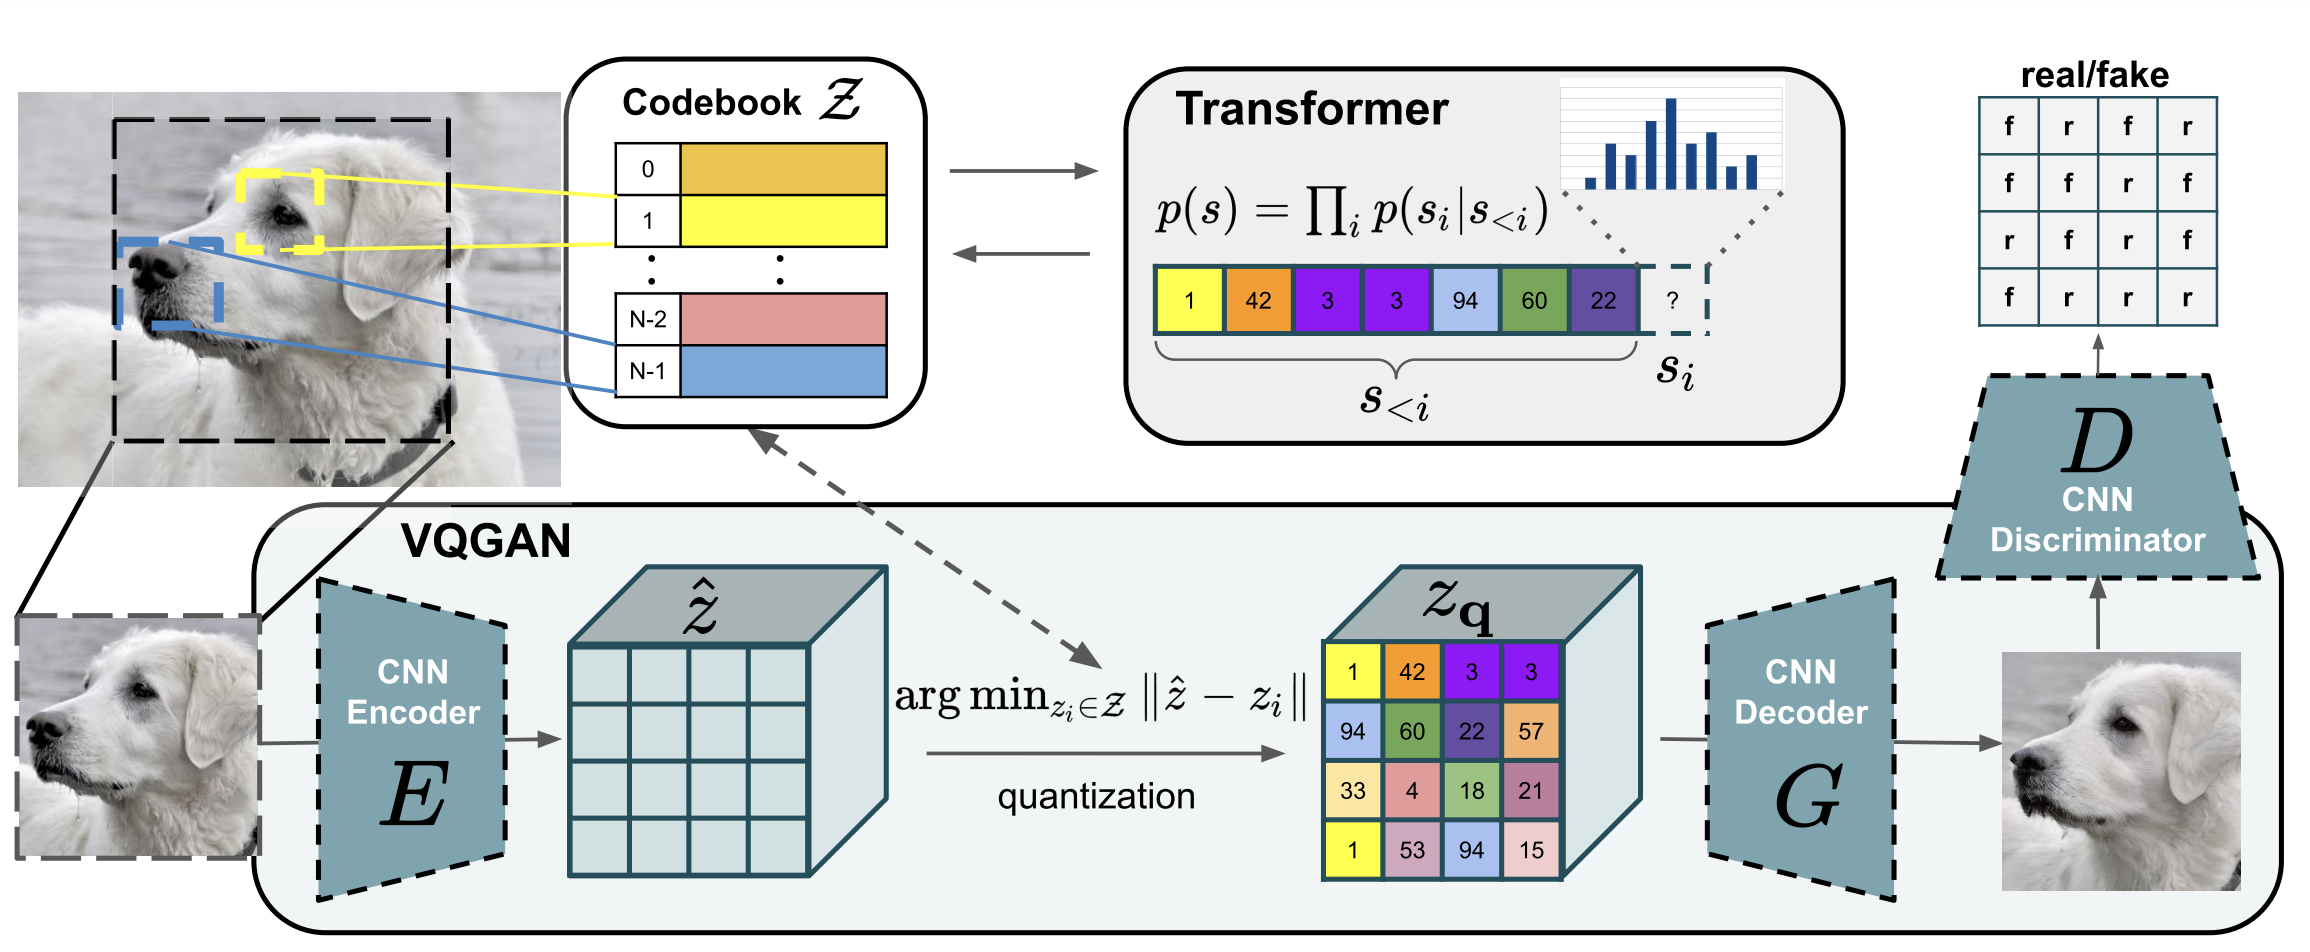
\includegraphics[width=0.8\textwidth]{images/vqgan_architecture.png}
    \caption{VQ-GAN architecture \cite{vqgan}. The bottom rectangular part is the VQ-VAE module with the addition of a descriminator $D$ (right), and the top part is the autoregressive transformer network that predicts the next code vector $s_i$ based on previous outputs $s_{<i}$.}
    \label{fig:vqgan_architecture}
\end{figure}

In the source code of VQ-GAN the researchers used the VGG16 \cite{vgg16} architecture as the backbone of the encoder and decoder networks, but they mentioned that other architectures can be used as well, depending on the generative task. In addition, the authors used the minGPT \cite{mingpt} architecture as the transformer module (more commonly known as GPT-2, which is based on the OpenAI's model GPT-1).

The non-differential operation of quantization is a problem we saw previously in VQ-VAE (subsection \ref{subsec:vqvae_vq}), and to solve this problem the authors said that they used the straight-through estimator \cite{ste} to backpropagate the gradients through the quantization process, similarly to VQ-VAE.






\subsection{Architecture}

THe architecture of VQ-GAN is shown in figure \ref{fig:vqgan_architecture}. The training involves feeding images $x \in X$ of size $x \in \mathbb{R}^{H \times W \times 3}$ \footnote[2]{The training dataset was of size $256 \times 256 \times 3$.} to the encoder $E$ to get the latent representation $\hat{z}$ of size $\hat{z} \in \mathbb{R}^{h \times w \times n_z}$, where $n_z$ is the dimension of each codebook vector. These representation are then quantisized by the VQ module to get the discrete latent representation $z_q \in \mathbb{R}^{h \times w \times n_z}$. This operation converts latent vectors to indencies of code vectors by nearest neighbor code vector (index in the codebook points to a code vector). Using $z_q$ vectors, the CNN decoder $G$ then reconstructs the image $\hat{x}$. A discriminator $D$ is used to distinguish between real and fake (generated) pixel patches of size 16x16. This module encourages the model to generate finer details and local patterns in the image, leading to better overall quality.

The autoregressive transformer is used to predict the embeddings $z_q$ and provide the decoder $G$ the nessessary information to generate a new image.




\subsection{Training}

The model is trained in two stages: in the first phase, the VQ-VAE module is trained to learn a discrete latent representation of the input data (learn the codebook), and the second phase trains the transformer module to predict the code vectors sequence that will be used to generate the output image.

The loss function of training the model to learn the codebook is given by: (similar to the VQ-VAE loss function in equation \ref{eq:vqvae_loss}):

\begin{equation}
    \mathcal{L}_{\text{VQ}} (E, G, \mathcal{Z}) = \Vert x - \hat{x} \Vert ^2 + \Vert \text{sg}[E(x)] - z_q \Vert ^2_2 +  \beta \Vert \text{sg}[z_q] - E(x) \Vert ^2_2
\end{equation}

where the first term is the MSE reconstruction loss, the second term is the quantization error, and the third term is the commitment loss. The reconstruction loss is intended to train the decoder $G$ to output (reconstruct latents $z_q$) images of similar distribution to the dataset. The quantization loss encourages the model to move the codebook vectors torwards the encoder outputs, to match the encoder's output distribution (gradients are calculated for $z_q$ and not $\text{sg}[E(x)]$ because of the stop gradient operation). The commitment loss encourages the encoder to "commit" to outputting embeddings that are close to the codebook vectors.

However, instead of the MSE loss, the authors used a perceptual loss \footnote[3]{Perceptual loss measures the difference between the high-level features of two images (a generated image and an image from the dataset). Typically the high-level features are extracted by pretrained CNNs.} and \textbf{introduced an adversarial training procedure with a patch-based discriminator $D$} that tries to distinguish between real and fake pixel patches of size 16x16 of an image. The loss function of the discriminator is given by:

\begin{equation}
    \mathcal{L}_{\text{GAN}}(\{E,G,Z\}, D) = [\log D(x) + \log (1-D(\hat{x}))]
\end{equation}

If $D$ outputs 1, then the image is from the dataset (real), and if it outputs 0, then the image is fake (generated by the decoder $G$). Just like in GAN, the discreiminator objective is to maximize the probability of assigning the correct label to the input image and in the loss function the first term encourages the discriminator to output 1 because $\log D(x)$ approaches 0 when $D(x)$ approaches 1, and the second term encourages the discriminator to output 0 for fake images because $\log (1-D(\hat{x}))$ approaches 0 when $D(\hat{x})$ approaches 0.

Combining both the VQ loss and the adversarial loss, the total loss function is given by:

\begin{equation}
    \mathcal{Q^*} = \arg \min_{E, G, Z} \max_D \mathbb{E}_{x \sim p(x)} [\mathcal{L}_{\text{VQ}} + \lambda \mathcal{L}_{\text{GAN}}]
\end{equation}

The $\lambda$ hyperparameter is used to balance the contribution of adversarial loss relative to the VQ loss.

\begin{figure}
    \centering
    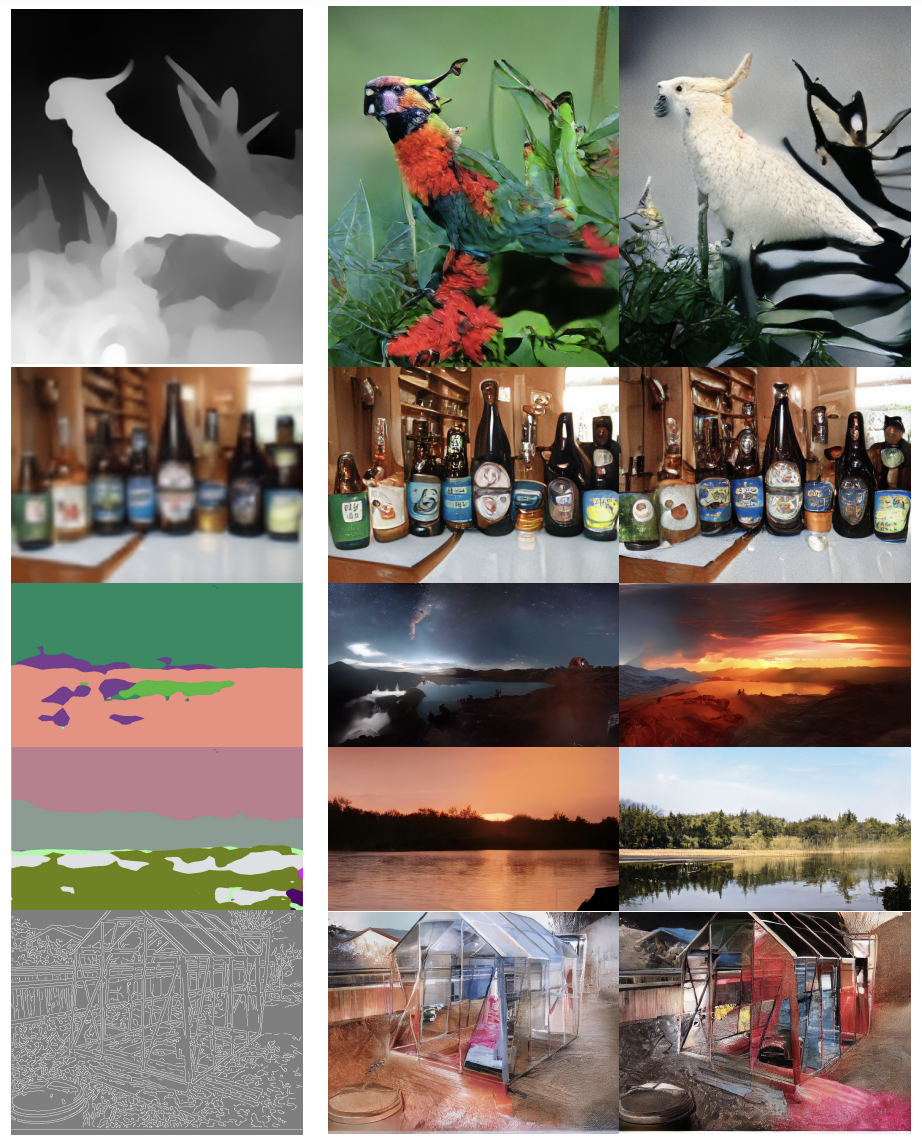
\includegraphics[width=0.5\textwidth]{images/vqgan_samples2.png}
    \caption{Samples generated by VQ-GAN by different tasks and different resolutions. From top to bottom: depth-to-image on RIN dataset, stochastic superresolution (super-resolution task) on RIN dataset, 3rd and 4th row are semantic synthesis (semantic masks) on S-FLCKR dataset, and bottom row are edge synthesis on IN dataset.}
\end{figure}





The second phase of the training involves maximizing the transformer objective. The transformer learns to predict the distribution of possible next indices, which allows us to directly maximize the log-likelihood (appendix \ref{appendix:likelihood_function}) of the data representation:

\begin{equation}
    \mathcal{L}_{\text{transformer}} = \mathbb{E}_{x \sim p(x)} [- \log p(x)]
\end{equation}

To summorize, the VQ-GAN model has 3 loss functions: the VQ loss (which trains the model to learn the codebook vectors), the adversarial loss (which trains the model to generate realistic images), and the transformer loss (which trains the model to predict the next code vector autoregressivly).







\subsection{Conditional generation}

% TODO: Finish
After the two-phase training is finished, the transformer is used to predict a sequence $s$ which is sequence of indencies to code vectors. Each token $s_i$ coresponds to an index in the codebook. So a code vector is autoregressivly predicted based on the previous tokens $s_{<i}$, which provides the nessessary embeddings $z_q$ for image synthesis ($p(s) = \prod_{i} p(s_i | s_{<i})$). If the image generation process involves a condition basis $c$, such as text, images, depth map, semantic layout or pose, then another VQ-GAN model is trained on these kind of tasks, which obtain a new codebook $Z_c$ which are the representation $r$ of $c$. Then, this representation is prepended to $s$ which restricts the computation of the negative log-likelihood to entries $p(s_i | s_{<i}, r)$. This new sequence is then given to the transformer in the first model to generate the image based on the condition $c$ (figure \ref{fig:vqgan_conditional_generation}).

\begin{figure}
    \centering
    \label{fig:vqgan_conditional_generation}
    \caption{The conditioned input sequence given to the transformer, based on the spatial condition information $c$. The middle rectangle represents a 'begin sequence' token.}
    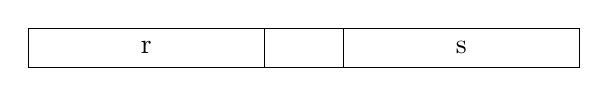
\begin{tikzpicture}
        \def \rectheight{0.5}

        % Draw the first rectangle
        \draw (0,0) rectangle (3,\rectheight);
        \node at (1.5,\rectheight / 2) {r};
        
        % Draw the middle rectangle
        \draw (3,0) rectangle (4,\rectheight);
        
        % Draw the third rectangle
        \draw (4,0) rectangle (7,\rectheight);
        \node at (5.5,\rectheight / 2) {s};
    \end{tikzpicture}
\end{figure}






\subsection{Sliding window technique for generating high-resolution images}

\begin{figure}
    \centering
    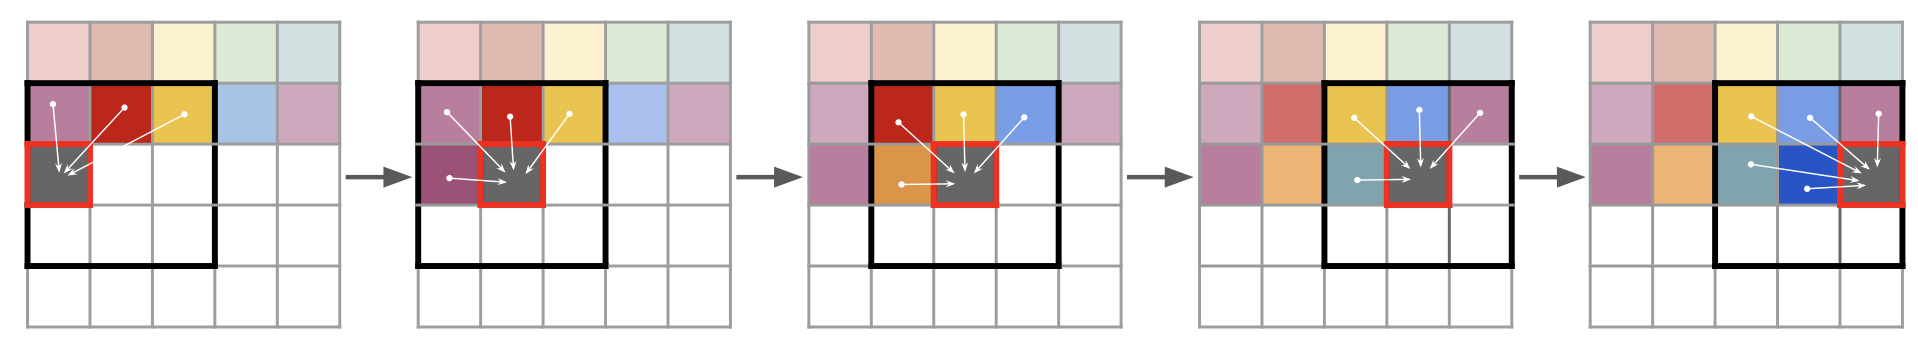
\includegraphics[width=0.5\textwidth]{images/vqgan_sliding_attention.png}
    \caption{Sliding window attention technique for generating high-resolution images. The output image is divided into patches of size 16x16=256 and by using attention mechanism, the transformer module is able to autoregressivly generate the next code vector $s_i$ based on the previous outputs $s_{<i}$ (the context).}
    \label{fig:vqgan_sliding_window}
\end{figure}

Due to the attention mechanism in transformers (quadratic computation for number of tokens, because each token requires attention to all other tokens), the model is limited in the size of the transformer sequence (in the paper they used 256 tokens). Although the encoder can reduce the dimentionality of images, the researchers noticed significant degration in generation quality. To solve this problem, they work patch-wise and crop input images to match the maximum token count in the transformer module.

To sample images, they also work patch-wise and the transformer autoregressivly predicts the next token based on the window context (figure \ref{fig:vqgan_sliding_window}).

